% !TeX spellcheck = en_US
\documentclass[letterpaper,12pt,twoside]{report}
\usepackage{fancyhdr}
\usepackage{fullpage}
\usepackage{tikz}
\usepackage{amsmath}
\usepackage{textcomp}

\begin{document}
	\pagestyle{fancy}
	\fancyhf{}
	\fancyhead[L]{Day 22}
	\fancyhead[R]{\textit{The Calendar Project}}
	\fancyfoot[L]{Citations Involved: none}
	
	% Problem
	\paragraph{Problem}
	\begin{quote}
		\textsf{In the figure, $\triangle RED$ is a right
			triangle with legs of length 6 yards and
			8 yards. Quadrilateral \textit{\textrm{BLUE}} is a
			square. What is the area of \textit{\textrm{BLUE}}?}
	\end{quote}
	
	% Graphics
	\begin{center}
		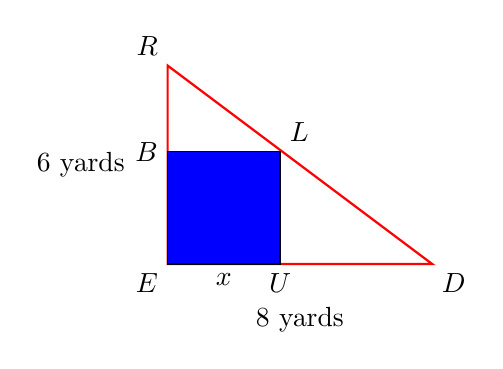
\begin{tikzpicture}[scale=0.42]
		\draw[thick][red] (0,6) -- (0,0) -- (8,0) -- cycle;
		\draw[fill=blue] (0,0) -- (3.4,0) -- (3.4,3.4) -- (0,3.4) -- cycle;
		
		\node[above left] at (0,6) {$R$};
		\node[below left] at (0,0) {$E$};
		\node[below right] at (8,0) {$D$};
		\node[left] at (0,3.4) {$B$};
		\node[above right] at (3.4,3.4) {$L$};
		\node[below] at (3.4,0) {$U$};
		\node[below] at (1.7,0) {$x$};
		
		\node[below] at (4,-1) {8 yards};
		\node[left] at (-1,3) {6 yards};
		\end{tikzpicture}
	\end{center}
	
	% Reasoning
	\paragraph{Reasoning}
	\begin{quotation}
		
		Let the side length of $BLUE$ be $x$ yards. It is shown above that $x=EU=UL=LB=BE$. By the SAP, $EU+UD=ED$; given that $ED$ has a length of 8 yards, $x+UD=8$ and thus $UD=8-x$. Given that $\triangle RED$ is a right triangle, $\angle RDE$ can be determined using $\arctan \frac{6}{8} \approx 36.87$\textdegree (3). Since a square is a parallelogram, its opposite sides are parallel (2); given that $\angle BED$ is a right angle, $\angle LUD$ is also a right angle by the Corresponding Angles Postulate (1); $\triangle LUD$ is therefore a right triangle. $\angle RDE \cong \angle LDU$ by the Reflexive Property; thus $LU=x=UD \tan \angle LDU=(8-x)\tan (\arctan \frac{6}{8})$. This is used to solve for $x$ as follows:
		
		\begin{center}
			\begin{tabular}{l | l}
				$x=(8-x) \cdot \frac{6}{8}$ & Simplify $\tan(\arctan ...)$ \\
				$x=6-\frac{6}{8}x$ & Apply the Distributive Property \\
				$\frac{14}{8}x=6$ & Add both sides by $\frac{6}{8}x$ \\
				$x=6 \cdot \frac{8}{14}$ & Multiply both sides by $\frac{8}{14}$ \\
				$x=\frac{24}{7}$ & Simplify
			\end{tabular}
		\end{center}
		
		The formula for the area of a square is $x^2$ where $x$ is its side length (4); therefore the area of $BLUE$ is $(\frac{24}{7})^2=\boxed{\dfrac{576}{49} \approx 11.755 \text{  yards}^2}$.
	\end{quotation}
	
	\paragraph{External References}
	
	\begin{enumerate}
		\item Textbook Ch. 3, Pg. 155: Corresponding Angles Postulate
		\item Textbook Ch. 6, Pg. 391: Properties of Parallelograms
		\item Textbook Ch. 8, Pg. 525: Trignometric Ratios
		\item Textbook Ch. 9, Pg. 589: Area of a Parallelogram
	\end{enumerate}
	
\end{document}